\documentclass{beamer}
\mode<beamer>{\usetheme{Madrid}}
\usepackage{graphicx} % Required for inserting images
\usepackage{eso-pic}
\usepackage[absolute,overlay]{textpos}
\setbeamertemplate{section in toc}[sections numbered]
\setbeamertemplate{subsection in toc}[ball unnumbered]
\setbeamertemplate{footline}
{
  \leavevmode%
  \hbox{%
  \begin{beamercolorbox}[wd=.5\paperwidth,ht=2.25ex,dp=1ex,center]{title in head/foot}%
    \usebeamerfont{title in head/foot}\insertshorttitle
  \end{beamercolorbox}%
  \begin{beamercolorbox}[wd=.5\paperwidth,ht=2.25ex,dp=1ex,center]{date in head/foot}%
    \usebeamerfont{date in head/foot}\insertshortdate{}\hspace*{2em}
    \insertframenumber{} / \inserttotalframenumber\hspace*{2ex} 
    \hspace*{6ex}
  \end{beamercolorbox}}%
  \vskip0pt%
}

\newcommand\AtPagemyUpperLeft[1]{\AtPageLowerLeft{%
\put(\LenToUnit{0.75\paperwidth},\LenToUnit{0.91\paperheight}){#1}}}
\AddToShipoutPictureFG{
  \AtPagemyUpperLeft{{
\includegraphics[width=2.5cm,keepaspectratio]{figure/uzh_logo_e_neg.eps}}}
}%



\title{Markowitz Portfolio Optimization with Inflation}
\author{Pablo Duce Cabeza, Djordje Nikolic, Sergey Mirzoev, Marc Tschudi}
\date{December 2023}

\begin{document}

\begin{frame}
\titlepage
\begin{center}
    
\includegraphics[width=2.5cm,keepaspectratio]{figure/uzh_logo_e_pos.eps}
\end{center}
\end{frame}


\begin{frame}
\frametitle{Outline}
\tableofcontents
\end{frame}

% \section{Introduction}
% \subsection{Sub a}
% \begin{frame}
% \frametitle{Introduction: Sub a}
% lorem
% \end{frame}

% \subsection{Sub b}
% \begin{frame}
% \frametitle{Introduction: Sub b}
% lorem ipsum
% \end{frame}

% \section{Approach}
% \begin{frame}
% \frametitle{Approach 1}
% Approach for Code
% \end{frame}

% \begin{frame}
% \frametitle{Approach 2}
% Approach for Portfolio Construction
% \end{frame}

% \section{PNL}
% \begin{frame}
% \frametitle{PNL}
% Insert PNL graph
% \end{frame}

\section{Abstract}

\begin{frame}{Abstract}
  \begin{itemize}
    \item Investigate the relationship between various asset classes and inflation.
    \item Analyse CPI, Oil, Gold, Bonds, Real Estate, Bitcoin, and S\&P 500.
    \item Develop a portfolio optimized for inflation protection.
  \end{itemize}
\end{frame}

\section{Introduction}

\begin{frame}{Introduction}
  \begin{itemize}
    \item Hypothesis: Certain assets have a higher correlation with inflation and therefore offer a natural hedge against inflation.
    \item Assets considered: TIPS, Gold, Real Estate, Oil, Stocks, Bonds, Bitcoin.
    \item Analysis involves exploring the relationship between inflation and selected assets.
  \end{itemize}
\end{frame}

\section{Methodology}

\begin{frame}{Methodology}
  \begin{itemize}
    \item Data collection using DataDownloader.
    \item Normalising returns and analysing correlations.
    \item Quantile-Quantile (Q-Q) plots for percentile analysis.
    \item Portfolio optimisation based on mean-variance.
  \end{itemize}
\end{frame}

\section{Results}

\begin{frame}{Results}
  \begin{itemize}
    \item Optimal portfolio weights and performance metrics.
    \item PnL generation based on optimal weights.
    \item Efficient Frontier analysis for risk-return trade-offs.
  \end{itemize}
\end{frame}

\begin{frame}{Results: KPIs}
The optimized portfolio exibits the following KPIs:
\begin{table}[H]
\centering
\begin{tabular}{ | m{7cm} | m{4cm} | }
 \hline
 \textbf{Measure} & \textbf{Result} \\
 \hline
 Expected Annual Return & 9.82\% \\ 
 \hline
 Risk (Annual standard deviation) & 19.96\% \\
 \hline
 Sharpe Ratio 0.4922 & 0.49 \\ 
 \hline
\end{tabular}
 \label{table:tab1}
 \caption{KPIs.}
\end{table}
\end{frame}



\begin{frame}{Results: Efficient Frontier}
The optimized portfolio lies on the efficient frontier:
  \begin{figure}
    \centering
    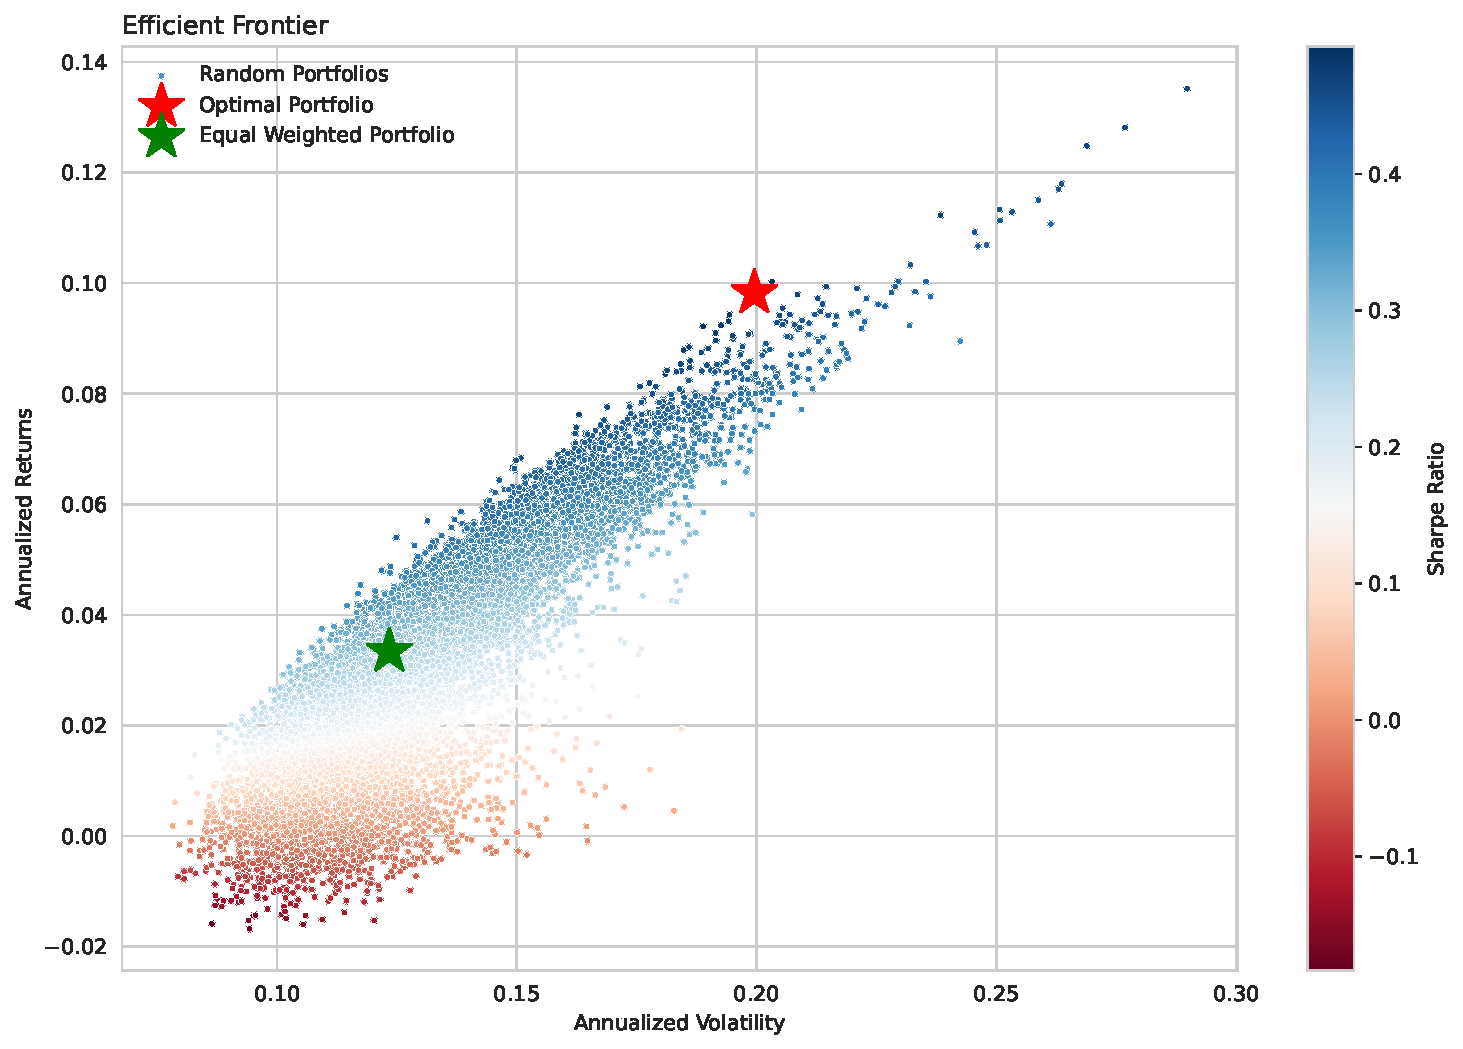
\includegraphics[width=0.75\textwidth]{paper/figure/Optimal_PF.pdf}
    \caption{Efficient Frontier}
  \end{figure}
\end{frame}

\begin{frame}{Results: Performance and Benchmark}
The optimized portfolio adjusted for the CPI outperforms the equally weighted CPI adjusted portfolio:
  \begin{figure}
    \centering
    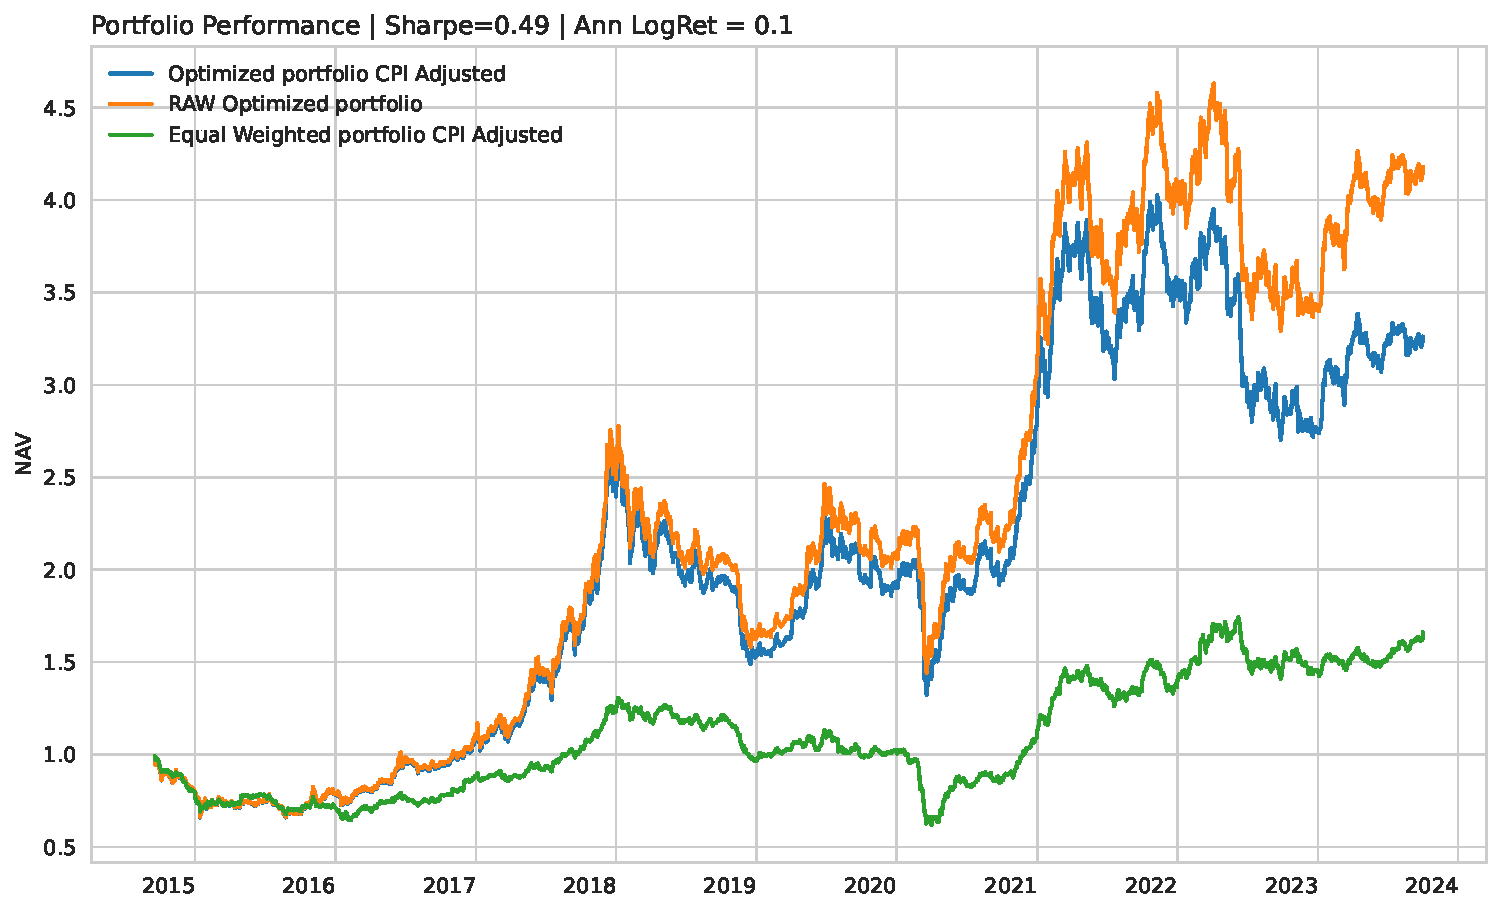
\includegraphics[width=0.75\textwidth]{paper/figure/PNL.pdf}
    \caption{Optimal Portfolio PnL}
  \end{figure}
\end{frame}

\end{document}
